\let\negmedspace\undefined
\let\negthickspace\undefined
\documentclass[journal]{IEEEtran}
\usepackage[a5paper, margin=10mm, onecolumn]{geometry}
%\usepackage{lmodern} % Ensure lmodern is loaded for pdflatex
\usepackage{tfrupee} % Include tfrupee package

\setlength{\headheight}{1cm} % Set the height of the header box
\setlength{\headsep}{0mm}     % Set the distance between the header box and the top of the text

\usepackage{gvv-book}
\usepackage{gvv}
\usepackage{cite}
\usepackage{amsmath,amssymb,amsfonts,amsthm}
\usepackage{algorithmic}
\usepackage{graphicx}
\usepackage{textcomp}
\usepackage{xcolor}
\usepackage{txfonts}
\usepackage{listings}
\usepackage{enumitem}
\usepackage{mathtools}
\usepackage{gensymb}
\usepackage{comment}
\usepackage[breaklinks=true]{hyperref}
\usepackage{tkz-euclide} 
\usepackage{listings}
% \usepackage{gvv}                                        
\def\inputGnumericTable{}                                 
\usepackage[latin1]{inputenc}                                
\usepackage{color}                                            
\usepackage{array}                                            
\usepackage{longtable}                                       
\usepackage{calc}                                             
\usepackage{multirow}                                         
\usepackage{hhline}                                           
\usepackage{ifthen}                                           
\usepackage{lscape}
\begin{document}

\bibliographystyle{IEEEtran}
\vspace{3cm}

\title{4.7.62}
\author{EE25BTECH11065 - Yoshita}
% \maketitle
% \newpage
% \bigskip
{\let\newpage\relax\maketitle}

\renewcommand{\thefigure}{\theenumi}
\renewcommand{\thetable}{\theenumi}
\setlength{\intextsep}{10pt} % Space between text and floats

\textbf{Question}:\\
Find the equation of the plane which passes through the point (5, 2, -4) and perpendicular to the line with direction ratios 2, 3, -1.\\
\bigskip

\textbf{Solution}:\\
The plane passes through a known point,
\[ \mathbf{A} = \myvec{5\\2\\-4} \]
The plane is perpendicular to a line with direction ratios (2, 3, -1). 
\[ \mathbf{n} = \myvec{2\\3\\-1} \]
The equation of a plane is given by the formula\[ \mathbf{n}^T (\mathbf{x} - \mathbf{A}) = 0\] where $\mathbf{x}$ is a general point $[x, y, z]^T$ on the plane.

Substituting the numerical values for our normal vector $\mathbf{n}$ and point $\mathbf{A}$:
\begin{align*}
    \myvec{2 & 3 & -1} \left( \myvec{x\\y\\z} - \myvec{5\\2\\-4} \right) &= 0 \\
    \implies \myvec{2 & 3 & -1} \myvec{x-5\\y-2\\z-(-4)} &= 0 \\
    \implies \myvec{2 & 3 & -1} \myvec{x-5\\y-2\\z+4} &= 0 \\
    \implies 2(x-5) + 3(y-2) - 1(z+4) &= 0 \\
    \implies 2x - 10 + 3y - 6 - z - 4 &= 0 \\
    \implies 2x + 3y - z &= 20
\end{align*}
Thus, the equation of the plane is $2x + 3y - z = 20$.
\begin{figure}[h!]
\begin{center}
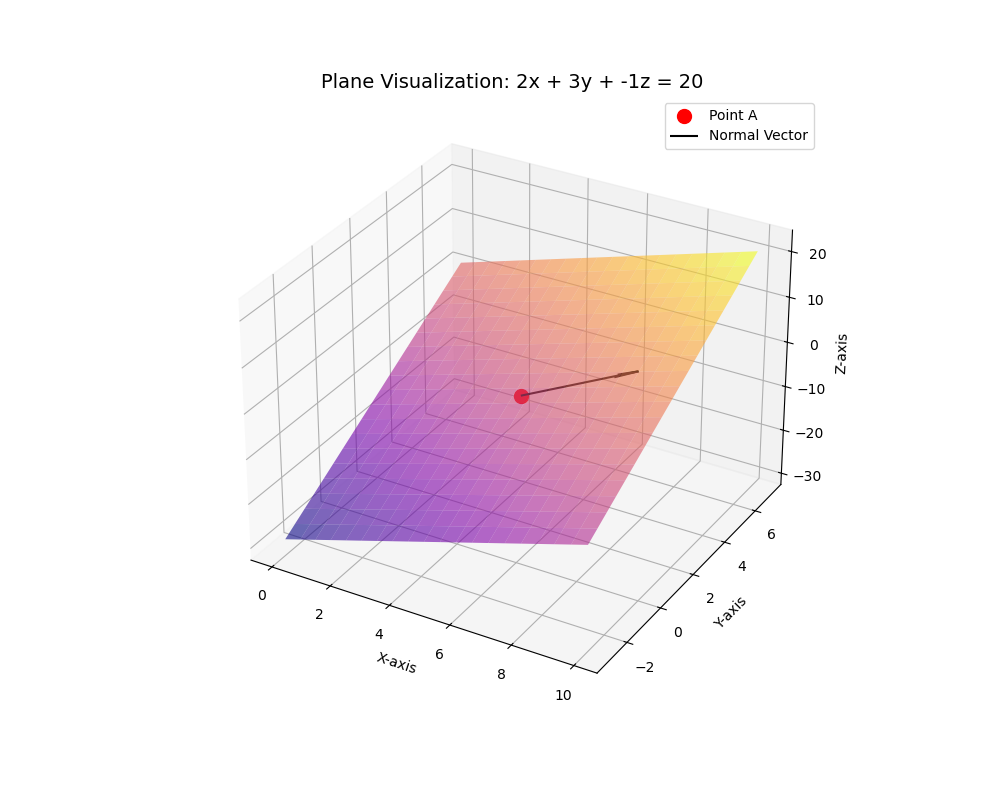
\includegraphics[width=\columnwidth]{figs/fig4.png}
\end{center}
\caption{A plane passing through point A with normal vector n.}
\label{fig:Fig.1}
\end{figure}
\end{document}


